\section{Methodology}
\label{sec3}

\noindent This chapter presents the design and implementation details of the proposed MAT4PM framework. 
% Specifically, Subsection~\ref{subsection31} introduces the overall system architecture and the core design principles. Subsection~\ref{subsection32} provides a formal definition of the optimal threshold and elaborates on the construction of the objective function. Subsection~\ref{subsection33} describes the data collection process.
\rev{
Specifically, Subsection~\ref{subsection31} introduces the overall system architecture and core design principles, Subsection~\ref{subsection32} formalizes the definition of the optimal threshold and the associated objective function, and Subsection~\ref{subsection33} details the data collection process.
}

\subsection{MAT4PM}
\label{subsection31}

\noindent This section presents a novel traffic monitoring approach that integrates P4-based proactive monitoring with machine learning techniques, termed MAT4PM (Machine Learning-Guided Adaptive Threshold Control for P4-Based Monitoring). 
MAT4PM addresses the limitations of static threshold strategies, which often fail to adapt to varying network conditions. 
By introducing a data-driven adaptive threshold control mechanism, MAT4PM enables switches to intelligently adjust monitoring thresholds based on real-time traffic characteristics, thereby reducing monitoring errors and communication overhead.

\begin{figure}[!t]
    \centering
    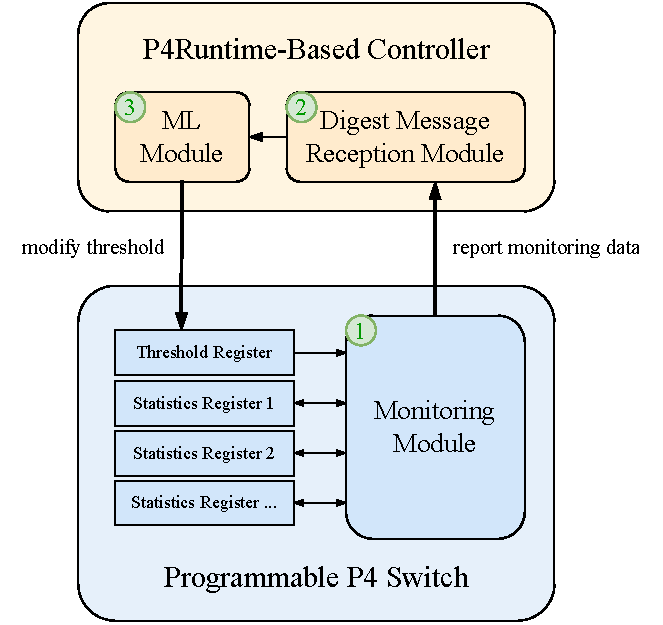
\includegraphics[width=0.45\textwidth]{./figures/arch.pdf}
    \caption{MAT4PM Architecture.}
    \label{arch}
\end{figure}

Figure~\ref{arch} illustrates the overall architecture of the MAT4PM system. 
The framework consists of three functional modules distributed across the data plane and the control plane, which collaborate to deliver efficient and intelligent traffic monitoring. 
The module numbers below correspond to those in the figure:

\begin{enumerate}
    \item \textbf{Monitoring Module}: Deployed on programmable P4 switches, this data plane component collects real-time traffic statistics and triggers reports when any monitored metric exceeds a predefined threshold.
    \item \textbf{Digest Message Reception Module}: Located on the controller based on P4Runtime~\cite{P4Runtime}, this module receives and processes statistical reports from switches and invokes the ML Module.
    \item \textbf{ML Module}: Responsible for inferring the optimal monitoring threshold based on the current traffic conditions and issuing the updated threshold to the switch for the next monitoring cycle.
\end{enumerate}

% These modules operate in a closed-loop workflow, where data plane events drive control plane decisions, and updated decisions are fed back to the data plane for continuous adaptation. 
\rev{These modules form a closed-loop workflow: data plane events trigger control plane decisions, which are then fed back to the data plane for continuous adaptation.} 
During system operation, the P4 switch continuously collects traffic statistics from passing packets, such as the number of packets and bytes within a fixed window. 
Simultaneously, it maintains a set of registers that store the current monitoring thresholds. 
These registers are used to determine whether an update should be triggered based on real-time traffic. 
When any monitored metric (e.g., packet or byte count within a window, or the elapsed time since the last report) exceeds its corresponding threshold, the switch immediately initiates a proactive reporting mechanism, sending a digest message containing the relevant statistics to the controller. 
Upon each reporting event, local counters are reset, initiating a new monitoring cycle and ensuring an event-driven, low-latency response mechanism.

Upon receiving digest messages from the switch, the controller first parses the report and extracts the traffic-related features. 
It then invokes a pre-trained machine learning model to predict the optimal threshold for the current network state. 
This prediction considers both monitoring accuracy and communication cost, striking a dynamic balance between precision and overhead. 
The newly predicted threshold is then written back into the relevant switch registers, allowing subsequent monitoring actions to proceed under updated conditions.

In subsequent algorithmic descriptions, experimental setups, and performance evaluations, we use the monitoring period threshold $prd_m$ as a representative example for triggering reporting actions. 
Specifically, during each monitoring interval, the system checks whether the time since the last report for a given flow exceeds its designated $prd_m$ threshold. 
If so, a new report is triggered. 
This time-based triggering mechanism is both simple and generalizable, making it suitable for various scenarios. 
Regarding the selected monitoring features, this work focuses on two fundamental yet critical traffic indicators: packets per second (pps) and bits per second (bps). 
These metrics are widely adopted in network performance analysis and anomaly detection, as they effectively capture dynamic traffic behaviors and provide highly relevant input features for subsequent error evaluation and threshold optimization.

To validate the feasibility of the proposed method and conduct functional testing, the system is implemented on BMv2 (Behavioral Model version 2)~\cite{BMv2}, the official open-source software switch for P4. 
\rev{
It is important to note that BMv2 primarily serves as a development and debugging platform and does not incorporate performance-oriented optimizations typically found in production-grade switching systems. 
Compared to optimized software switches such as Open vSwitch (OVS)~\cite{OVS}, as well as hardware-based programmable switching platforms including Tofino ASIC~\cite{TFTG}, BMv2 exhibits substantially lower packet processing throughput and higher per-packet processing latency. 
This performance gap arises from the interpretive execution model and lack of hardware acceleration in BMv2, which distinguishes it from both high-performance software data planes and specialized programmable hardware. 
Accordingly, the experimental evaluation in this study emphasizes functional correctness and feasibility analysis of the proposed mechanisms, rather than throughput-oriented benchmarking or performance comparison under line-rate deployment conditions.
}

\subsubsection{Monitoring Threshold Configuration and Retrieval}

Algorithm~\ref{algo_thld} illustrates how the MAT4PM system stores and retrieves the monitoring period threshold $prd_m$. 
Since the P4 language does not support the direct definition or access of global variables, the system employs registers to preserve state across packets. 
This design enables each monitored flow to independently maintain its current threshold configuration, adhering to the constraints of the P4 language while supporting efficient per-flow indexing and updates via flow identifiers.

Specifically, the system defines a register array named $prds_m$ to store the reporting period thresholds for all monitored flows, where each entry corresponds to a specific flow. 
Let $N_{flow}$ denote the total number of monitored flows, and the register must support indexable access to up to $N_{flow}$ distinct entries. 
To ensure correct address computation, the index width is set at compile time to $\lceil \log_2 N_{flow} \rceil$, guaranteeing a unique mapping for each flow identifier within the supported range. 
This mechanism ensures that each flow has an independent and dynamically adjustable monitoring period, which is a critical component enabling MAT4PM's fine-grained adaptive monitoring capabilities.

\begin{algorithm}[!t]
    \caption{Monitoring threshold configuration and retrieval}
    \label{algo_thld}
    \begin{algorithmic}[1]
        \STATE // The \textbf{register} below is used to store the monitoring period thresholds.
        \STATE \textbf{register}$<$bit$<$48$>$, bit$<\lceil \log_2 N_{flow} \rceil>>$($N_{flow}$) $prds_m$;
        \STATE
        \STATE // The \textbf{function} below retrieves the monitoring period threshold.
        \STATE bit$<$48$>$ get\_thld(in bit$<\lceil \log_2 N_{flow} \rceil> flow\_num$) \{
        \STATE \hspace{1em} bit$<$48$>$ $prd_m$;
        \STATE \hspace{1em} $prds_m$.read($prd_m$, $flow\_num$);
        \STATE \hspace{1em} return $prd_m$;
        \STATE \}
    \end{algorithmic}
\end{algorithm}

\subsubsection{Monitoring Data Report}

In programmable P4 switches, there are typically two mechanisms for transmitting data plane information to the control plane: the packet-in mechanism, where a complete packet carrying the required information is encapsulated and sent to the controller; and the digest mechanism, which transmits only selected structured fields in the form of a lightweight message. 
% In the MAT4PM system, the digest mechanism is adopted for reporting monitoring results from the data plane, based on comprehensive considerations of performance and communication efficiency which are illustrated as follows.
\rev{In the MAT4PM system, the digest mechanism is adopted for reporting monitoring results from the data plane, due to its advantages in performance and communication efficiency, as discussed below.}

The packet-in approach generally forwards the entire packet, including the header and payload, as a distinct stream message under P4Runtime. 
Although this method offers flexibility, it incurs high communication overhead, especially in network monitoring scenarios where frequent reporting is required. 
Such frequent transmissions significantly burden bandwidth and control channels. 
Moreover, each packet-in message is triggered as an independent event, limiting opportunities for aggregation and batching, and consequently affecting scalability under high-volume reporting. 
In contrast, the digest mechanism allows switches to transmit only essential monitoring fields, such as statistical counters or metadata, without carrying full packet content, thereby substantially reducing message size. 
Additionally, multiple digest messages can be automatically aggregated by the P4Runtime server at the switch side and forwarded to the controller in batch mode. 
This batching capability notably improves transmission efficiency. 
More importantly, digest functions can only be invoked in the ingress control path, aligning seamlessly with MAT4PM's monitoring logic, which is also deployed in the ingress stage. 
Considering all these factors, the digest mechanism represents the optimal strategy for implementing event-driven reporting in MAT4PM.

Algorithm~\ref{algo_report} describes the procedure through which MAT4PM uses digest messages to report monitoring data. 
Each digest encapsulates the unique identifier of the monitored flow ($flow\_num$) along with its associated metrics, including the total number of bytes and packets, as well as the elapsed time since the last report.

\begin{algorithm}[!t]
    \caption{Monitoring data report}
    \label{algo_report}
    \begin{algorithmic}[1]
        \STATE // The \textbf{registers} below are used to store monitoring data.
        \STATE \textbf{register}$<$bit$<$32$>$, bit$<\lceil \log_2 N_{flow} \rceil>>$($N_{flow}$) $pkts$;
        \STATE \textbf{register}$<$bit$<$32$>$, bit$<\lceil \log_2 N_{flow} \rceil>>$($N_{flow}$) $bytes$;
        \STATE \textbf{register}$<$bit$<$48$>$, bit$<\lceil \log_2 N_{flow} \rceil>>$($N_{flow}$) $times$;
        \STATE
        \STATE // Digest Message Struct.
        \STATE \textbf{struct} reported\_data \{
        \STATE \hspace{1em} bit$<\lceil \log_2 N_{flow} \rceil>$ flow\_num;
        \STATE \hspace{1em} bit$<$48$>$ timestamp\_delta;
        \STATE \hspace{1em} bit$<$32$>$ reported\_pkt;
        \STATE \hspace{1em} bit$<$32$>$ reported\_byte;
        \STATE \}
        \STATE
        \STATE // The \textbf{function} below is used to send digest message.
        \STATE void report\_to\_controller(
        \STATE \hspace{1em} in bit$<\lceil \log_2 N_{flow} \rceil>$ $flow\_num$,
        \STATE \hspace{1em} in bit$<$48$>$ $timestamp\_delta$
        \STATE ) \{
        \STATE \hspace{1em} reported\_data data;
        \STATE \hspace{1em} data.flow\_num = flow\_num;
        \STATE \hspace{1em} data.timestamp\_delta = timestamp\_delta;
        \STATE \hspace{1em} $pkts$.read(data.reported\_pkt, $flow\_num$);
        \STATE \hspace{1em} $bytes$.read(data.reported\_byte, $flow\_num$);
        \STATE \hspace{1em} digest$<$reported\_data$>$(1, data);
        \STATE \}
    \end{algorithmic}
\end{algorithm}

\subsubsection{Data Plane Monitoring Mechanism}

Figure~\ref{ingress} illustrates the internal processing workflow for traffic monitoring within the packet processing pipeline of a programmable P4 switch. 
The monitoring logic is primarily implemented in the ingress control block and comprises two critical actions: one responsible for flow monitoring (denoted as the Monitoring Action) and the other for triggering the reporting mechanism (denoted as the Reporting Action). 
Together, these ensure real-time statistics updates and event-driven monitoring data reporting.

\begin{figure}[!t]
    \centering
    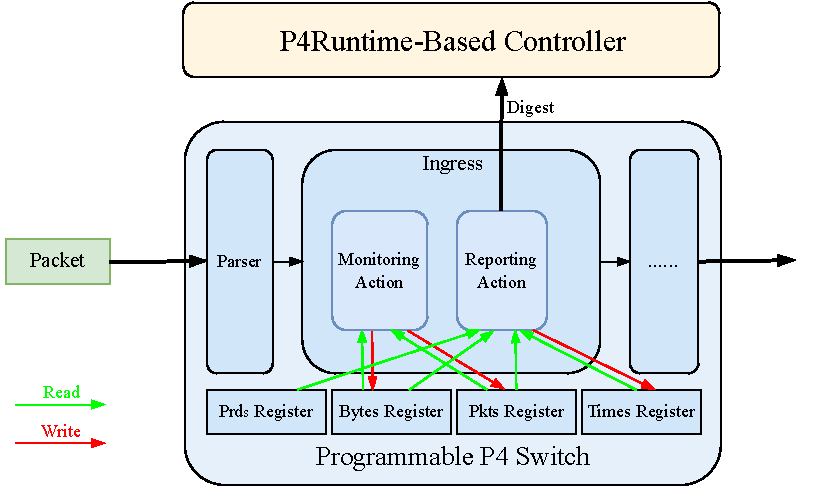
\includegraphics[width=0.5\textwidth]{./figures/ingress.pdf}
    \caption{Processing pipeline in data planes.}
    \label{ingress}
\end{figure}

Upon arrival at the switch, a packet is first parsed by the P4 parser, which extracts header fields layer by layer. 
The packet then proceeds to the ingress match-action stage, where it is matched against flow table entries. 
If a match is found, the system executes the monitoring action. 
This action uses the flow identifier as an index to access two monitoring registers: $bytes$ and $pkts$, which accumulate the total number of bytes and packets received for the corresponding flow, respectively. 
After incrementing these values based on the current packet, the updated counters are written back to the registers, enabling per-packet granularity in flow statistics collection.

Following the update of monitoring registers, the packet processing enters the reporting action. 
At this stage, the system reads the last report timestamp for the current flow from the $times$ register. 
It then calculates the time elapsed since the last report using the current system timestamp, which is obtained from the standard ingress metadata (\texttt{standard\_metadata.ingress\_global\_timestamp}). 
The reporting threshold for this flow, denoted as $prd_m$, is retrieved from the $prds$ register. 
If the elapsed time exceeds or equals $prd_m$, the reporting condition is satisfied, and a digest message is immediately generated to send the current flow statistics to the controller. 
Simultaneously, the monitoring counters in $bytes$ and $pkts$ are reset to zero to begin a new monitoring interval, and the current timestamp is written back to $times$ as a reference for the next report cycle.

This monitoring and reporting mechanism relies heavily on stateful registers and an event-driven design, enabling responsive data plane monitoring with minimal latency. 
It fully leverages the programmability of P4 and provides a high-quality data foundation for the controller's subsequent machine learning-based threshold adaptation. 
The corresponding P4 pseudocode implementation is presented in Algorithm~\ref{algo_ingress}.

\begin{algorithm}[!t]
    \caption{Data plane monitoring mechanism}
    \label{algo_ingress}
    \begin{algorithmic}[1]
        \STATE \textbf{control} Ingress(inout headers hdr,
        \STATE \hspace{1em} inout metadata meta,
        \STATE \hspace{1em} inout standard\_metadata\_t standard\_metadata) \{
        \STATE \hspace{1em} // The \textbf{action} below is the monitoring operation for flows.
        \STATE \hspace{1em} \textbf{action} monitor\_flow(in bit$<\lceil \log_2 N_{flow} \rceil>$ $flow\_num$) \{
        \STATE \hspace{2em} bit$<$32$>$ pkt, byte;
        \STATE \hspace{2em} $pkts$.read(pkt, $flow\_num$);
        \STATE \hspace{2em} $bytes$.read(byte, $flow\_num$);
        \STATE \hspace{2em} pkt = pkt + 1;
        \STATE \hspace{2em} byte = byte + standard\_metadata.packet\_length;
        \STATE \hspace{2em} $pkts$.write($flow\_num$, pkt);
        \STATE \hspace{2em} $bytes$.write($flow\_num$, byte);
        \STATE \hspace{1em} \}
        \STATE \hspace{1em} // The {\bf action} below determines whether to report the monitoring data based on the monitoring threshold.
        \STATE \hspace{1em} {\bf action} report\_flow(in bit$<\lceil \log_2 N_{flow} \rceil>$ $flow\_num$) \{
        \STATE \hspace{2em} bit$<$48$>$ time, now, delta;
        \STATE \hspace{2em} $times$.read(time, $flow\_num$);
        \STATE \hspace{2em} now = standard\_metadata.ingress\_global\_timestamp;
        \STATE \hspace{2em} delta = now - time;
        \STATE \hspace{2em} // Function get\_thld() is implemented in Algorithm~\ref{algo_thld}.
        \STATE \hspace{2em} \textbf{if} (delta $>=$ get\_thld($flow\_num$)) \{
        \STATE \hspace{3em} // The implementation of report\_to\_controller() is presented in Algorithm~\ref{algo_report}.
        \STATE \hspace{3em} report\_to\_controller($flow\_num$, delta);
        \STATE \hspace{3em} // Reset the monitoring data of this flow.
        \STATE \hspace{3em} $pkts$.write($flow\_num$, 0);
        \STATE \hspace{3em} $bytes$.write($flow\_num$, 0);
        \STATE \hspace{3em} // Update the last reported time of this flow.
        \STATE \hspace{3em} $times$.write($flow\_num$, now);
        \STATE \}\}\}
    \end{algorithmic}
\end{algorithm}

\subsubsection{Control Plane Decision Processing Mechanism}

Figure~\ref{controller} illustrates the core internal processing workflow of the MAT4PM controller. 
Within the system architecture, the \textit{Digest Message Reception Module} is responsible for receiving and handling digest messages transmitted from the data plane. 
Upon receiving a new report, this module parses the message and extracts essential monitoring features, including the flow identifier, the number of packets, the total byte count, and the elapsed time since the last report. 
% These extracted features are then assembled into a standardized input vector and passed to a pre-trained machine learning model for inference, which outputs the optimal monitoring interval threshold for the given flow. 
\rev{These extracted features are assembled into a standardized input vector and passed to a pre-trained machine learning model for inference. The model outputs the optimal monitoring interval threshold for the given flow.} 
Once the predicted threshold is obtained, the controller proceeds to synchronize this value with the data plane to update the local monitoring policy at the switch level.

\rev{To mitigate unnecessary consumption of control plane bandwidth caused by frequent minor updates that contribute little to monitoring effectiveness}, MAT4PM integrates a threshold update suppression mechanism. 
Specifically, the controller maintains a local hash table \rev{to store the most recently enforced monitoring thresholds for all active flows}. 
When a new threshold is predicted, \rev{it is compared against the previously applied value associated with the same flow}. 
\rev{A control plane update is triggered only if the relative difference between the two exceeds a configurable suppression margin (e.g., 10\%). 
This margin is a tunable system parameter that can be adjusted according to deployment requirements, traffic dynamics, and control plane resource constraints, rather than a fixed constant embedded in the design.}

\rev{
If the suppression condition is satisfied, a \texttt{write\_register} instruction is issued to update the monitoring threshold stored in the corresponding switch register. 
Otherwise, the update is deferred, allowing the data plane to continue operating under the existing configuration. 
By filtering out insignificant threshold variations caused by short-term traffic fluctuations or minor prediction noise, this mechanism reduces control plane communication overhead and improves system stability, while preserving the ability to react to meaningful traffic changes. 
The complete control logic, encompassing digest message reception, feature extraction, machine learning-based inference, and conditional threshold updates, is summarized in Algorithm~\ref{algo_controller}.
}

\begin{figure}[!t]
    \centering
    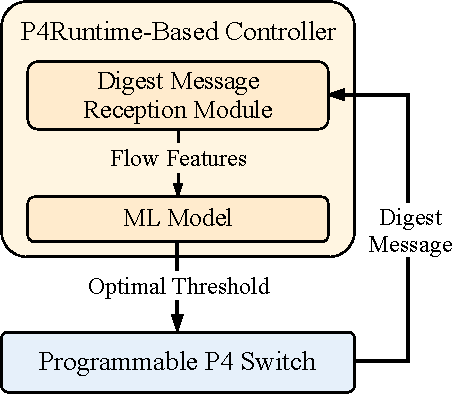
\includegraphics[width=0.32\textwidth]{./figures/controller.pdf}
    \caption{Internal processing workflow of a controller.}
    \label{controller}
\end{figure}

\begin{algorithm}[!t]
    \caption{Control plane decision processing mechanism}
    \label{algo_controller}
    \begin{algorithmic}[1]
        \WHILE{true}
        \STATE // Wait and receive digest messages.
        \STATE $msg$ $\Leftarrow$ \texttt{get\_digest\_message()};
        \STATE // Parse $msg$ to extract the monitoring data.
        \STATE $flow\_num,\ \Delta t,\ packets,\ bytes \Leftarrow msg$.\texttt{parse()};
        \STATE $pps,\ bps \Leftarrow packets / \Delta t,\ (bytes \times 8) / \Delta t;$
        \STATE // Construct feature vector $\mathbf{x}$.
        \STATE $\mathbf{x} \Leftarrow \{bps,\ pps\}$;
        \STATE // Predict optimal threshold.
        \STATE $prd_m^* \Leftarrow \texttt{ML\_Model.Predict}(\mathbf{x})$;
        \IF{$\lvert ( prd_m^* - old\_prd_m ) / old\_prd_m \rvert > 10\%$}
        \STATE // Update the threshold for this flow.
        \STATE \texttt{write\_register($flow\_num$, $prd_m^*$)};
        \ENDIF
        \ENDWHILE
    \end{algorithmic}
\end{algorithm}

\subsection{Optimal Threshold Definition}
\label{subsection32}

\noindent To construct a labeled dataset suitable for training a machine learning model, it is first necessary to rigorously define the concept of an optimal monitoring period threshold. 
This section derives the definition starting from basic traffic rate metrics, followed by error modeling, communication cost estimation, and finally the formulation of a composite cost function for determining the optimal threshold.

Two fundamental traffic rate indicators are considered: bit rate (bps, bits per second) and packet rate (pps, packets per second). 
For traffic observed over a continuous time window, the rates are defined as:
\begin{equation}
    bps = \frac{\text{Total Bytes} \times 8}{\Delta t} ,
\end{equation}
\begin{equation}
    pps = \frac{\text{Total Packets}}{\Delta t} ,
\end{equation}
where $\Delta t$ denotes the duration of the observation interval in seconds, while Total Bytes and Total Packets refer to the number of bytes and packets recorded during this interval, respectively. 
In practice, the reported rate by the switch may deviate from the ground-truth rate derived via offline analysis. 
To quantify such deviations, two separate relative error metrics are defined:

\begin{equation}
    \label{eq:err_bps}
    E_{bps} = \left| \frac{bps_{reported} - bps_{true}}{bps_{true}} \right| ,
\end{equation}

\begin{equation}
    \label{eq:err_pps}
    E_{pps} = \left| \frac{pps_{reported} - pps_{true}}{pps_{true}} \right| ,
\end{equation}
where $bps_{reported}$ and $pps_{reported}$ denote the bit rate and packet rate reported by the switch, while $bps_{true}$ and $pps_{true}$ are their respective ground-truth values obtained from packet trace analysis. 
A simple linear combination is used to define the overall monitoring error:

\begin{equation}
    \label{eq:E}
    E = E_{bps} + E_{pps} .
\end{equation}

The monitoring threshold $prd_m$ (in milliseconds) not only affects the accuracy of measurements but also directly influences the communication overhead between the data and control planes. 
Smaller thresholds lead to more frequent reporting, increasing control channel load. 
The reporting frequency per unit time is thus defined as:
\begin{equation}
    \label{eq:C}
    C = \frac{1}{prd_m} .
\end{equation}
To integrate $C$ with $E$ in a unified optimization framework, normalization is required. 
A maximum reporting frequency $C_{max} = 50$ is adopted as the normalization constant, implying that up to 50 monitoring reports per second are permitted per switch. 
This upper bound is based on practical engineering observations regarding the capacity of SDN controllers and the tolerance of control plane bandwidth. 
Exceeding this threshold has been shown to cause undesirable effects such as increased controller CPU load, control message queuing, packet loss, and latency. 
Therefore, $C_{max} = 50$ reflects a realistic limit for maintaining system responsiveness without overburdening the control infrastructure. 
The normalized communication cost is computed as:
\begin{equation}
    \label{eq:Cnorm}
    C_{norm} = \frac{C}{C_{max}} ,
\end{equation}
ensuring that $C_{norm} \in [0, 1]$, which enables consistent weighting with the monitoring error term.

The overall cost of a monitoring strategy is then formulated as:
\begin{equation}
    \label{eq:cost(prd_m)}
    cost(prd_m) = \alpha \cdot E + \beta \cdot C_{norm}, \quad \alpha + \beta = 1 ,
\end{equation}
where $\alpha$ and $\beta$ are tunable hyperparameters that control the trade-off between monitoring accuracy and communication overhead. 
In subsequent experiments, $\alpha = 0.6$ and $\beta = 0.4$ are used, slightly favoring accuracy over overhead reduction.

The optimal monitoring threshold $prd_m^*$ is defined as the value that minimizes the overall cost for a given traffic sample. 
An exhaustive search method is employed to evaluate all candidate thresholds within a predefined interval of $[20, 1500]$ milliseconds, covering the practical range from high-frequency to low-frequency monitoring. 
The optimal threshold is formally expressed as:
\begin{equation}
    prd_m^* = \arg\min_{prd_m \in [20, 1500]} cost(prd_m) .
\end{equation}
This definition enables the labeling of each flow sample with its corresponding optimal monitoring period, thereby facilitating the construction of a high-quality supervised learning dataset essential for subsequent model training.

\subsection{Data Processing}
\label{subsection33}

\noindent
% To construct a high-quality labeled dataset suitable for training machine learning models, this section provides a detailed description of the data acquisition, processing, and labeling workflow.
\rev{This subsection describes the data acquisition, processing, and labeling workflow used to construct the training dataset.}

During the initialization of the BMv2 software switch using the \texttt{simple\_switch\_grpc} command, the \texttt{--pcap} parameter is configured to specify the output directory for packet capture (PCAP) files. 
This setting enables the switch to record all transiting packets during runtime into standardized PCAP format files. 
PCAP is a widely adopted data interchange format in network analysis, extensively used in diagnostics, security auditing, and performance evaluation. 
It preserves complete packet-level information, including protocol headers, payloads, timestamps, and packet lengths. 
Due to its broad compatibility, PCAP data can be parsed and analyzed using mainstream tools such as Wireshark, Tshark, and Tcpreplay, making it suitable for offline traffic reconstruction and anomaly detection research.

Once a traffic batch is generated, the corresponding PCAP file is extracted as the ground-truth reference. 
For an accurate replay that aligns with the original capture rate, packet playback is conducted using Scapy, which enables fine-grained control over the transmission interval of individual packets. 
Unlike tools such as Tcpreplay, which transmits packets as fast as possible, or playcap, which is primarily designed for loopback testing scenarios, Scapy allows for precise timing replication of the original traffic. 
This ensures that the replayed packet stream closely matches the temporal dynamics of the original capture, thereby preserving the fidelity of flow rates within each monitoring window.

Under the premise of accurately replayed traffic, the system then performs multiple experimental cycles under varying monitoring thresholds $prd_m$, ensuring that each configuration is evaluated under identical traffic conditions. 
For a given threshold, the number of bytes and packets in each reporting window is extracted from the PCAP file to compute the true bit rate and packet rate. 
These values are then compared against the switch-reported metrics to compute the monitoring error using the previously defined error functions. Subsequently, the communication cost and the total cost are computed using the normalized formulas introduced earlier.

For each fixed traffic rate, multiple candidate thresholds are evaluated. 
The corresponding total costs are recorded, and the threshold that minimizes the cost function is selected as the optimal monitoring threshold $prd_m^*$ for that traffic condition. The system then transitions to a new traffic configuration and repeats the same procedure until the entire range of predefined traffic conditions is covered.

The resulting dataset consists of three attributes: the reported bit rate (\texttt{reported\_bps}), the reported packet rate (\texttt{reported\_pps}), and the corresponding optimal monitoring threshold (\texttt{optimal\_prdm}). 
These two reported metrics are selected as input features because, in practical deployment scenarios, the switch can only provide flow statistics it measures directly. 
True rates (such as \texttt{true\_bps} and \texttt{true\_pps}) are only available during offline dataset construction and cannot be accessed during real-time operation. 
Hence, the model training process strictly emulates real-world conditions by using only observable switch-reported data, ensuring the deployability and operational feasibility of the trained model.

Through this rigorous data processing and labeling pipeline, a diverse and well-annotated dataset is constructed, spanning a wide range of traffic conditions and embedding optimal threshold labels. 
This provides a solid foundation for training and evaluating machine learning models in subsequent sections. The overall process is summarized in Algorithm~\ref{algo_collection}.

\begin{algorithm}[!t]
    \caption{Data processing}
    \label{algo_collection}
    \begin{algorithmic}[1]
        \STATE \textbf{Initialize:} candidate thresholds $prds_m = [20, 1500]$ ms
        \FOR{each traffic rate setting}
        \STATE Start BMv2 with PCAP recording enabled.
        \STATE Replay captured packets at original timing using Scapy.
        \FOR{each threshold $prd_m$ \textbf{in} $prds_m$}
        \STATE Set $prd_m$ as the current monitoring threshold.
        \STATE Monitor and record reported \texttt{bps}, \texttt{pps} during replay.
        \STATE Compute real \texttt{bps} and \texttt{pps} from PCAP ground truth.
        \STATE Calculate error metric $E$ according to Eq.~\ref{eq:E}.
        \STATE Calculate communication cost $C$ according to Eq.~\ref{eq:Cnorm}.
        \STATE Evaluate total cost $cost(prd_m)$ according to Eq.~\ref{eq:cost(prd_m)}.
        \ENDFOR
        \STATE Find $prd_m^* = \arg\min cost(prd_m)$ over all candidates.
        \STATE Store sample: $\{\texttt{reported\_bps}, \texttt{reported\_pps}\} \rightarrow prd_m^*$.
        \ENDFOR
    \end{algorithmic}
\end{algorithm}
